\chapter{Traballo Realizado}
\label{chap:Traballo Realizado}

\lettrine{N}{este} apartado presentarase o traballo realizado, comezando por unha vista xeral do proceso, 
seguido dunha explicación dos diferentes módulos desenvolvidos e a súa interacción, así como os conxuntos de datos empregados.
Finalmete, presentaranse os resultados obtidos acompañados dunha análise dos mesmos.
\section{Vista Xeral}
\label{sec:VistaXeral}


\section{Conxuntos de datos}
\label{sec:Conxuntos de datos}

\subsection{FIRE}
\label{subsec:FIRE}

\cite{FIRE} composto por 134 pares de imaxes de retinas, con un tamaño de 2912 × 2912 pixels e un \gls{FOV} de 45◦× 45◦.
 Están clasificadas en 3 categorías según o grado de superposición e a presenza de diferencias anatómicas: textit{S}, textit{P} e textit{A}.

 \begin{figure}[ht]
    \centering
    \setlength{\tabcolsep}{8pt} % Adjust column spacing
    \begin{tabular}{|c|c|c|c|}
        \hline
        \textbf{Categoría} & \textbf{Nº de pares de imaxes} & \textbf{Superposición (\%)} & \textbf{Diferenzas Visuais} \\
        \hline
        \textbf{\textit{\textsf{S}}} & 71 & > 75 & Non \\
        \hline
        \textbf{\textit{\textsf{P}}} & 49 & < 75 & Non \\
        \hline
        \textbf{\textit{\textsf{A}}} & 14 & > 75 & Si \\
        \hline
    \end{tabular}
    \caption{Clasificación dos pares de imaxes en categorías.}
    \label{tab:categorias}
\end{figure}

Inclúe 10 puntos de referencia para cada imaxe, que se utilizan para a avaliación do rexistro, así como unha máscara por cada imaxe que indica a localización dos píxeles con información de cor.

\begin{figure}[ht]
    \centering
    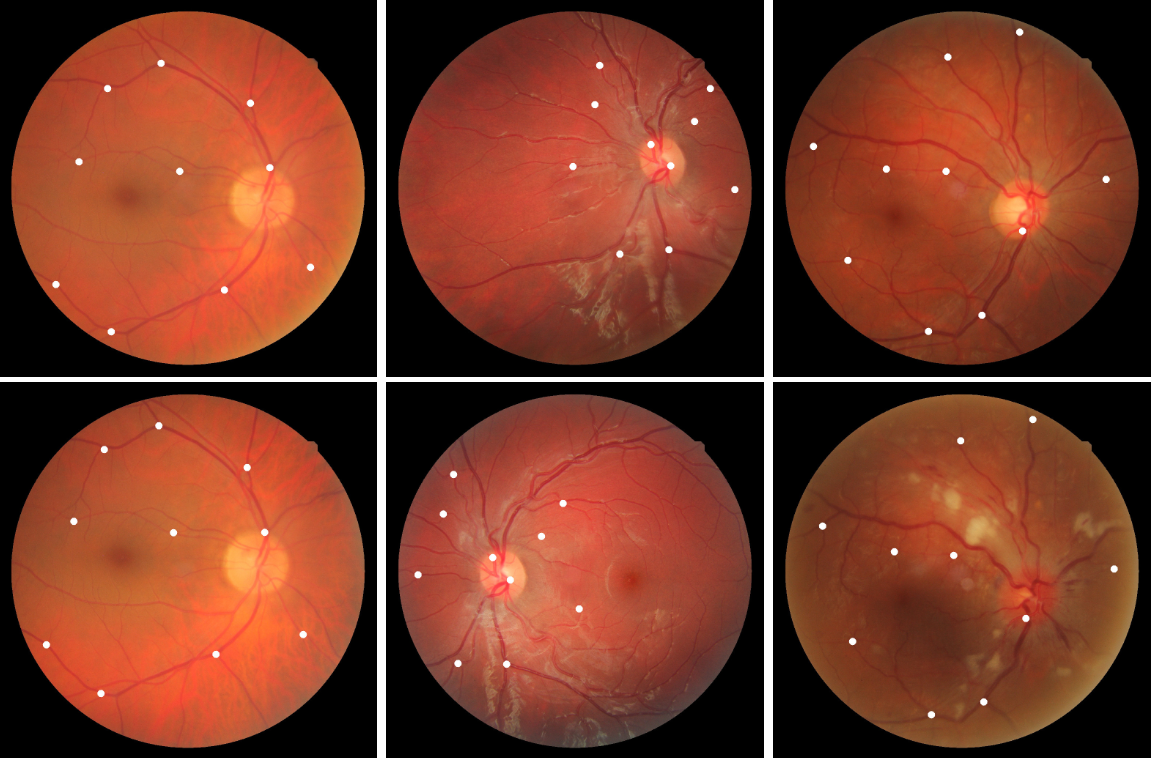
\includegraphics[width=0.8\textwidth]{imaxes/fire-ej.png}
    \caption{Exemplo de imaxes do conxunto de datos FIRE \cite{FIRE} cos puntos de control indicados. De esquerda a dereita, categorías \textit{\textsf{S}}, \textit{\textsf{P}}, \textit{\textsf{A}} .}
    \label{fig:fire_ej}
\end{figure}

\subsection{RFMID}
\label{subsec:RFMID}

O conxunto de datos RFMiD \cite{RFMiD} proporciona 3200 imaxes de fondo de ollo en cor etiquetadas en normal ou anormal. 
Tamén proporciona etiquetas para 45 diferentes enfermidades/anomalías anotadas por expertos.

Para utilizalo neste traballo, seleccionamos unha submostra e xeramos transfomacións aleatorias. Gardamos as imaxes orixinais e as transformadas así como as matrices de transformación asociadas para a posterior avaliación.
Tamén se divide entre transfomacións de cor e de xeometría.

\dots preguntar 

\section{Avaliación}
\label{sec:Avaliación}

Utilizamos o método de evaluación proposto por FIRE \cite{FIRE},
creando un gráfico onde o eixo x representa o valor do límite de erro e o eixo y mostra a porcentaxe de pares de imaxes que foron rexistrados con éxito para cada límite de erro

O error de rexistro calcúlase ca distancia media entre os puntos correspondentes na imaxe fixa e móbil (cj, rj).
Cando o erro de rexistro entre un par de imaxes está por debaixo do límite, considérase que o rexistro foi exitoso e viceversa. Isto dá lugar a unha curva monótona continua que reflicte a relación entre a taxa de éxito e a precisión obxectivo, evitando así a necesidade de establecer un limiar arbitrario. 
Estes gráficos utilízanse para ilustrar a precisión do rexistro tanto para individuais como para o conxunto completo de datos.

Esta métrica facilita a comparación entre distintos métodos competidores e permite seleccionar o máis axeitado segundo a precisión desexada.

Mentres que FIRE xa provee os puntos de referencia para a avaliación, RFMID non o fai.
Polo tanto, para RFMID, utilizamos o mesmo método de avaliación, pero xerándo os puntos manualmente cubrindo toda a imaxe.

\begin{figure}[ht]
    \centering
    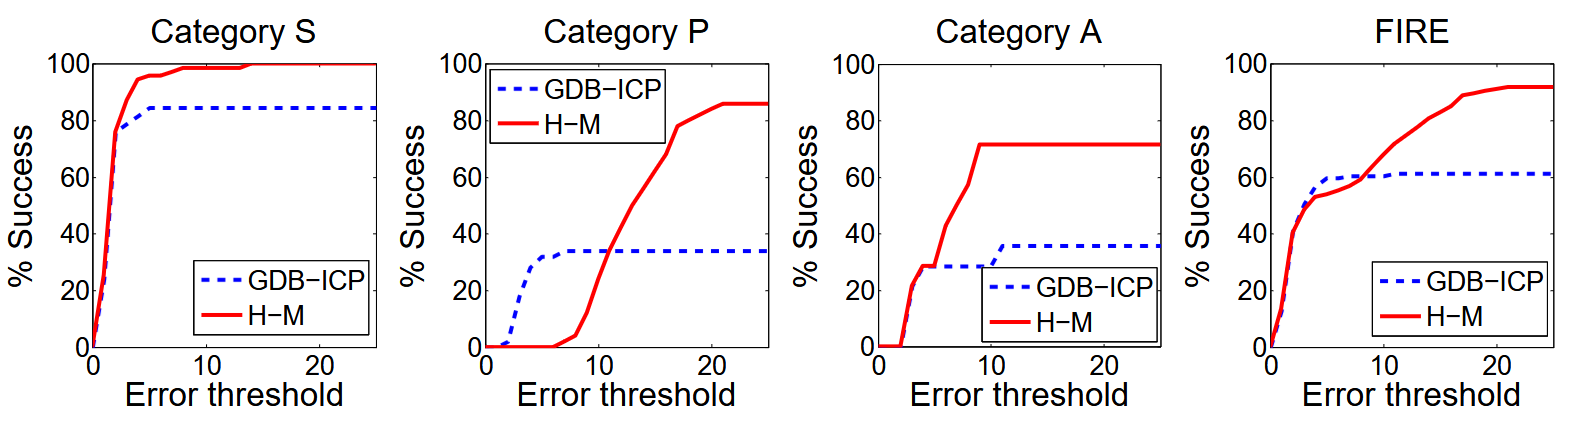
\includegraphics[width=0.8\textwidth]{imaxes/fire_aval.png}
    \caption{Gráfico de avaliación FIRE, \cite{FIRE}}
    \label{fig:fire_aval}
\end{figure}


\section{Discusión}
\label{sec:Discusión}